% ======================= Pre-Amble =========================
      
%Format
\documentclass[11pt, oneside]{article}   	% use "amsart" instead of "article" for AMSLaTeX format 
                     						%imports package {article} and specify option(s) [11pt, oneside]
\usepackage{geometry}                		% See geometry.pdf to learn the layout options. There are lots. 
    \geometry{letterpaper}                   		% ... or a4paper or a5paper or ... 
    %\geometry{landscape}                		% Activate for rotated page geometry

\usepackage[parfill]{parskip}    		        % Activate to begin paragraphs with an empty line rather than an indent

    %Colours
    \usepackage{graphicx, subcaption}
    \usepackage[usenames, dvipsnames]{color}     % font colour:    \textcolor{<colour>}{text}
          									%highlight text:  \colorbox{<color>}{text}
    \usepackage{soul}						%highlight text: \hl{}     %only  yellow								
    									%list of colours: https://www.sharelatex.com/learn/Using_colours_in_LaTeX
    									
    %Bullets
    \usepackage{enumerate}     %specify type of enumeration: \being{enumerate}[<type of enumeration>]
    
    %Footnote Spacing
    \setlength{\footnotesep}{0.4cm}                  %specify spacing b/w footnotes
    \setlength{\skip\footins}{0.6cm}                    % space b/w footnotes and textbody


%Mattematics
    %American Mathematics Society packages
    \usepackage{amsmath}	   %math
    \usepackage{amssymb}       %symbols
    \usepackage{amsthm}          %theorems

    %QED
    \newcommand*{\QEDA}{\hfill\ensuremath{\blacksquare}}         %make qed filled square:    \QEDA
    \newcommand*{\QEDB}{\hfill\ensuremath{\square}}               %make qed empty square: \QEDB 
    
    \renewcommand\qedsymbol{\ensuremath{\blacksquare}}		%Proof environment


%Figures
\usepackage{caption}
\captionsetup[figure]{labelfont=bf}    %make figure labels boldface
\captionsetup[table]{labelfont=bf}     %make table labels boldface

\usepackage[hidelinks]{hyperref}                % Allows for clickable references

    %Tables
    \usepackage[none]{hyphenat}                    % Stops breaking-up words in a table (i.e. no hyphens)                                                             
    
    \usepackage{array}   
    \newcolumntype{x}[1]{>{\centering\let\newline\\\arraybackslash\hspace{0pt}}p{#1}}       %center fixed column width: x{<len>}                      
    \newcolumntype{$}{>{\global\let\currentrowstyle\relax}}                                                   % let us apply things (e.g. bold/italicize) to entire row            
    \newcolumntype{^}{>{\currentrowstyle}}
    \newcommand{\rowstyle}[1]{\gdef\currentrowstyle{#1} #1\ignorespaces}
    
    %Images
    \graphicspath{ {images/} }                          %directory that your images are located in within your current directory
    
    %Diagrams
    \usepackage[latin1]{inputenc}
    \usepackage{tikz}
    \usepackage{tkz-berge}
    \usetikzlibrary{shapes,arrows}


%Bibliography
\usepackage[numbers,sort&compress]{natbib}   %for multiple references: sorts  (i.e. [1,2] NOT [2, 1] )
                                           				  %                                     compresses (i.e. [1-3] )
\usepackage[nottoc]{tocbibind}                            %add bibliography to table of contents


%Miscellaneous
\usepackage{dirtytalk}    %quotations: use \say  


%================== Header & Footer =========================
\usepackage{fancyhdr}
\usepackage{lastpage}      %ensures you can reference LastPage (i.e. Page 2 of 10)

\renewcommand{\headrulewidth}{0.4pt}		%Decorative Header line: thickness={0.4pt}
\renewcommand{\footrulewidth}{0.4pt}		%Decorative Footer line: thickness={0.4pt}

\setlength{\headheight}{13.6pt} 		%space b/w top of page & header
\setlength{\headsep}{0.3in}		%space b/w page header and body

%Make Header & Footer    
\pagestyle{fancy}
    \lhead{Stephanie Knill} 		% controls the left corner of the header
    \chead{} 					% controls the center of the header
    \rhead{} 					% controls the right corner of the header
    \lfoot{} 					% controls the left corner of the footer
    \cfoot{Page~\thepage\ of \pageref{LastPage}} 				% controls the center of the footer
    												%Page~\thepage\  if just want Page x
    \rfoot{}			 		% controls the right corner of the footer

% =============================== Document ===================================
\begin{document}

% Title Page
\title{MATH 302 --- Assignment 4 \\
\line(1,0){360} \\              %(slope x, y){length of line}
}
\author{
Stephanie Knill \\
54882113 \\
Due: February 10, 2016}

\date{}                   % Activate:  display a given date (e.g. {August 4} ) or no date (empty {} )
                                    %No activate: display current date
\maketitle

%\thispagestyle{empty}                   %Remove header from this (first) page. Change empty -> plain to keep numbering
%								-> Doesn't matter in this case (b/c title page)
%\cleardoublepage


% ================= Questions ================

\section*{Question 1: Section 4.1 \#32}

\begin{enumerate}[\quad (a)]
	\item Let $E$ be event that road 1 is clear and $F$ be the event that road 2 is clear. Thus the probability of each road being passable is $P(E) = p$ and $P(F) = q$. When the system's components are in \textit{series}, the reliability of them can be computed as follows:
	$$P(W \rightarrow T) = P(E \cap F)$$
Since events $E$ and $F$ are independent, the \textit{intersection} of the events is equal to the probability of each event occurring. Thus
	\begin{align*}
		P(E \cap F) & = P(E) \cdot P(F)\\
		& = pq 
	\end{align*}
	\item In the case where the system's components are in \textit{parallel}, the reliability of them is the \textit{union} of the two events:
	\begin{align*}
		P(W \rightarrow T) & = P(E \cup F) \\
		& = P(E) + P(F) - P(E \cap F) \\
		& = p + q - pq
	\end{align*}
	\item In this graph depicting the driving routes from Woodstock to Tunbridge, we now have 4 possible paths we can take such that we start at Woodstock and end in Tunbridge, and we do not use any edge (road) more than once. These will be represented by $E_1$, the path $W \rightarrow C \rightarrow T$, $E_2$, the path $W \rightarrow C \rightarrow D \rightarrow T$, $E_3$, the path $W \rightarrow D \rightarrow T$, and $E_4$, the path $W \rightarrow D \rightarrow C \rightarrow T$. Let $p=.8, q=.9$, and $r=.95$. Then we have $P(E_1)=P(E_3)=pq=.72$, $P(E_2) = p^2r = 0.608$, and $P(E_4)=q^2r=0.7695$.
	
	To compute the reliability of this graph, we have
	\begin{align*}
		P(W \rightarrow T) & = 1 - P(\text{no passable paths})\\
		& = 1 - P(\overline{E_1} \cap \overline{E_2} \cap \overline{E_3} \cap \overline{E_4}) \\
	\end{align*}
	Since each road being passable is independent, we have that $E_i$ and $E_j$ are independent for all $i \neq j$, $i, j \in \{1,2,3,4\}$. Thus we can rewrite our equation as:
	\begin{align*}
		P(W \rightarrow T) & = 1 - P(\overline{E_1}) \cdot P(\overline{E_2}) \cdot P(\overline{E_3}) \cdot P(\overline{E_4}) \\
		& = 1 - (1-P(E_1)) \cdot (1-P(E_2)) \cdot (1-P(E_3)) \cdot (1-P(E_4)) \\
		& = 1 - (1 - .72) \cdot (1 - .0608) \cdot (1- .72) \cdot (1-.7695) \\
		& \approx .9929
	\end{align*}

\end{enumerate}


\section*{Question 2: Section 4.1 \#43}

Let $Y$ be the random variable that gives the number of times the Yankees win a game in a series of length $n=7$. Since the Yankees can win the world series by either winning 4, 5, 6 or 7 games, the probability of them winning the series is
	\begin{align*}
		P(Y \geq 4) = P(Y=4) + P(Y=5)+P(Y=6)+P(Y=7) \\
	\end{align*}
	
Computing each separately, we have
	\begin{align*}
		P(Y=4) & = {n \choose k} \cdot p^k q^{n-k} \\
		& = {7 \choose 4} (.6)^4 (.4)^3 \\
		& \approx 0.2903
	\end{align*}
However, due to the greyscale of existence that is a student during midterm season, the remaining computations were done in Python (Figure \ref{Q2}). 
    \begin{figure}[h]                                         
    \begin{center}
        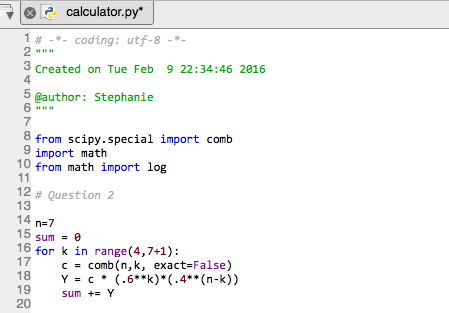
\includegraphics[width=.8\textwidth]{calculator.png}  
        \caption{Computation for $P(Y\geq 4)$ in Question 2.} 
        \label{Q2} 
    \end{center}
    \end{figure}
This gave a final value of $P(Y \geq 4) \approx 0.710208$.

\section*{Question 3: Section 4.1 \#49}
Let $H$ be the event that a coin is tossed and is Heads, with probability $P(H) = p_i$, for urn $i \in \{1,2\}$. Then in scenario (a) where we randomly select one of the two urns and flip both coins, we have 
	$$P(HH) = \frac{1}{2} p_1^2 + \frac{1}{2} p_2^2 = \frac{1}{2} (p_1^2+p_2^2)$$
and in scenario (b) where we flip one coin from each urn
	$$P(HH) = p_1 \cdot p_2$$
Since $p_1 \neq p_2$, then
	\begin{align*}
		(p_1 - p_2)^2 & > 0 \\
		p_1^2 - 2p_1p_2 + p_2^2 & > 0 \\
		p_1^2 + p_2^2 > 2p_1p_2 \\
		\frac{1}{2} (p_1^2 + p_2^2) > p_1p_2 \\
	\end{align*}
and we can conclude that the probability in scenario (a) is always greater than the probability in scenario (b) for all values of $p_1$ and $p_2$, thereby making scenario (a) the best choice.



\section*{Question 4: Section 5.1 \#6}

Let $X_1, \ldots , X_n$ be $n$ mutually independent random variables uniformly distributed on integers 1 to $k$. Let $Y$ denote the minimum of the $X_i$'s. Then the distribution of $Y$ can be expressed as
	$$P(Y=j) = P(Y > j-1) - P(Y > j),  \text{ where } 1<j<k $$
Since $min(X_1, \ldots, X_n) > j$ holds true exactly when $X_i > j$ for all $i \in \{1,\ldots,n\}$, we can calculate each component separately by
	\begin{align*}
		P(min(X_1, \ldots X_n) > j) & = P(X_1 > j)\cdot P(X_2 > j) \cdots P(X_n > j) \\
		& = \frac{k-j}{k} \cdot  \frac{k-j}{k} \cdots  \frac{k-j}{k} \\
		& = \Big(\frac{k-j}{k}\Big)^n \\
		& = \frac{(k-j)^n}{k^n} \\
	\end{align*}
and
	\begin{align*}
		P(min(X_1, \ldots X_n) > j-1) & = P(X_1 > j-1)\cdot P(X_2 > j-1) \cdots P(X_n > j-1) \\
		& = \frac{k-(j-1)}{k} \cdot \frac{k-(j-1)}{k} \cdots \frac{k-(j-1)}{k} \\
		& = \Big(\frac{k-(j-1)}{k}\Big)^n \\
		& = \frac{(k-(j-1))^n}{k^n} \\
	\end{align*}
Plugging this back into our original equation we have
	\begin{align*}
		P(Y=j) & =  \frac{(k-(j-1))^n}{k^n} -\frac{(k-j)^n}{k^n} \\
	\end{align*}
\section*{Question 5: Section 4.1 \#15}

\textbf{Conjecture:} For a geometric random variable $X$ of parameter $p$ and for non-negative integers $m$ and $n$, we have that
	$$P(X > n+m \mid X > m) = P(X > n)$$
	
\textbf{Proof}
	\begin{align*}
		P(X > n+m \mid X > m) & = \frac{P((X > n+ m) \cap (X > m))}{P(X > m)} \\
		& = \frac{P(X > n+ m)}{P(X > m)} \\
		& = \frac{(1-p)^{n+m}}{(1-p)^m} \\
		& = (1-p)^n \\
		& = P(X > n)
	\end{align*}
	\QEDA
	
\section*{Question 6: Section 5.1 \#14}

Let $X$ be the number of people with a particular rare blood type, with parameter $p= 1/1000$.

\begin{enumerate}[\quad (a)]
	\item For $n=10,000$, the probability of no person having this blood type is
		\begin{align*}
			P(X=0) & = {n \choose k} p^k q^{n-k} \\
			& = {10000 \choose 0} (1/1000)^0 \cdot (999/1000)^{10000} \\
			& = 4.517 \times 10^{-5}
		\end{align*}
	\item To find an $n$ such that the probability of at least one person has a rare blood type in a population is greater than 1/2 can be computed as follows:
		\begin{align*}
			P(X\geq 1) & = 1 - P(X=0)\\
			& = 1- {n \choose 0} p^0 q^{n} \\
			& = 1 - q^n
		\end{align*}
	Since $P(X \geq 1) > 1/2$
		\begin{align*}
			1 - q^n > 1/2 \\
			q^n < 1/2 \\
			\ln(q^n)> \ln(1/2) \\
			n > \frac{\ln(1/2)}{\ln(q)} \\
			n > 692.8 \\
			n = 693
		\end{align*}
\end{enumerate}


\section*{Question 7: Section 5.1 \#35}

Let $S$ be the number of brass turnbuckles manufactured and $D$ the number of those that are defective. A sample of $s$ items is drawn without replacement. Let $X$ be a random variable that gives the number of defective items in the sample. Let $p(d) = P(X = d)$.
\begin{enumerate}[\quad (a)]
	\item \textbf{Conjecture:}
	$$p(d) = \frac{{D \choose d}{S-D \choose s-d}}{{S \choose s}}$$
	
	\textbf{Proof}
	The probability that in a given sample $s$ that exactly $d$ items are defective can be expressed as
		$$P(X=d) = \frac{\text{\# ways sample has $d$ defective}}{\text{total \# ways draw sample $s$}}$$
	Computing the numerator, we have that the total number of ways to choose a sample $s$ from a population of $S$ items is ${S \choose s}$.
	
	For the denominator, we must choose $d$ defective items from a total of $D$ items; in other words, we have ${D \choose d}$ possible combinations. Of the remaining $S-D$ items in our set that are not defective, we must choose a sample of $s-d$ items. This gives us ${S-D \choose s-d}$. Thus the denominator is given by ${D \choose d}{S-D \choose s-d}$.
	
	Combining them all we have
		$$P(X=d) = p(d) = \frac{{D \choose d}{S-D \choose s-d}}{{S \choose s}}$$
	\QEDA
\end{enumerate}



\section*{Question 8}

\textbf{Proposition:} Let $X$ be a binomial random variable of parameters $n,p$. Then the value of $k$ that maximizes $P(X=k)$ is
$$\left \lfloor{(n+1)p}\right \rfloor $$

\textbf{Proof}

\begin{align*}
	\frac{P(X=k)}{P(X=k-1)} & = \frac{{n \choose k} \cdot p^k (1-p)^{n-k}}{{n \choose k-1} \cdot p^{k-1} (1-p)^{n-(k-1)}}\\
	& = \frac{{n \choose k} \cdot p}{{n \choose k-1}(1-p)}\\
\end{align*}
Here
	\begin{align*}
	\frac{{n \choose k}}{{n \choose k-1}} & = \frac{n!}{k! (n-k)!} \cdot \frac{(k-1)! (n-k+1)!}{n!} \\
	& = \frac{n+1}{k} - 1\\
\end{align*}
Substituting this back in
	\begin{align*}
		\frac{P(X=k)}{P(X=k-1)} & = \Big(\frac{n+1}{k} - 1 \Big) \cdot \frac{p}{(1-p)}\\
	\end{align*}
Since we want to find a $k$ such that $\frac{P(X=k)}{P(X=k-1)} \geq 1$
	\begin{align*}
		\frac{n+1}{k} - 1 & \geq \frac{(1-p)}{p}\\
		\frac{n+1}{k} \geq \frac{1}{p} \\
		k & \leq (n+1)p \\
	\end{align*}
Since $k \in \mathbb{Z}$ and we wish to maximize $P(X=k)$, we can conclude that
	$$k = \left \lfloor{(n+1)p}\right \rfloor $$
	
\QEDA


\end{document} 